\documentclass[times, utf8, seminar, numeric]{fer}
\usepackage{booktabs}
\usepackage{listings}
\usepackage{color}
\usepackage{url}
\usepackage{amsmath}
\usepackage{color, colortbl}
\usepackage{csvsimple}
\usepackage[group-separator={,}]{siunitx}
\usepackage{afterpage}

\definecolor{mygreen}{rgb}{0,0.6,0}
\definecolor{mygray}{rgb}{0.5,0.5,0.5}
\definecolor{mymauve}{rgb}{0.58,0,0.82}
\definecolor{gray1}{rgb}{0.93,0.93,0.93}

\lstset{ %
  backgroundcolor=\color{white},   % choose the background color
  basicstyle=\footnotesize,        % size of fonts used for the code
  breaklines=true,                 % automatic line breaking only at whitespace
  captionpos=b,                    % sets the caption-position to bottom
  commentstyle=\color{mygreen},    % comment style
  escapeinside={\%*}{*)},          % if you want to add LaTeX within your code
  keywordstyle=\color{blue},       % keyword style
  stringstyle=\color{mymauve},     % string literal style
}

\begin{document}

\title{Očitavanje rukom pisanih slova}
\author{Filip Gulan}
\voditelj{doc. dr. sc. Marko Čupić}

\maketitle
\tableofcontents

\chapter{Uvod}
Očitavanje slova je problem koji se rješava već dugi niz godina. Još od 1980-ih godina, početkom ere računala, počeli su se razvijati prvi programi koji bi zamijenili čovjeka u raznim operacijama, pa tako i u očitavanju slova. Primjena je bila razna, od očitavanja brojeva računa u bankama do očitavanja poštanskih brojeva prilikom sortiranja pisama.

Kroz ovaj rad prikazana je izgradnja jednog takvog sustava za prepoznavanje rukom pisanih slova koji bi bio unaprjeđenje istog iz rada \cite{seminar}. Sustav, kao i onaj iz prije navedenoga rada, koristi konvolucijsku neuronsku mrežu iste arhitekture no uz nešto drugačiji algoritam učenja te poboljšan skup podataka za učenje. Također, prikazana je i implementacija spomenutog sustava na uređajima sa zaslonom osjetljivim na dodir, gdje korisnik, umjesto s tipkovnicom, unosi znakove crtanjem po zaslonu uređaja.

U ostatku rada bit će opisan sam sustav i arhitektura. Zatim postupak učenja istog, te primjena u vidu prepoznavanja rukom nacrtanih znakova na uređajima sa zaslonom osjetljivim na dodir.

\chapter{Učenje i rezultati}
Za potrebe ovog rada izgrađen je sustav za klasifikaciju rukom pisanih slova hrvatske i engleske abecede uz dodatak znaka ''-'' koji se temelji na konvolucijskoj neuronskoj mreži. Sama mreža je izgrađena, učena i evaluirana korištenjem radnog okvira \emph{Keras}. \emph{Keras} je radni okvir napisan u programskom jeziku \emph{Python} koja nudi vrlo jednostavno programsko sučelje za izgradnju neuronskih mreža i širok spektar algoritama za učenje iste uz dodatne mogućnosti poput augmentacije podataka tokom samog učenja koja je korištena za potrebe ovog rada.

\section{Skup podataka}

Za potrebe učenja klasifikatora, to jest konvolucijske neuronske mreže, prikupljen je skup podataka od \num{16000} slika slova hrvatske abecede i znakova, i to \num{7750} velikih i \num{7750} malih slova te \num{500} primjera znaka "-".

Skup podataka je podijeljen na 63 razreda, gdje svaki razred određuje jedan znak. Pa su tako iz hrvatske abecede izbačena slova koja se mogu dobiti kombinacijom više znakova (lj, nj i dž) te su, uz spomenuti znak "-", dodana i slova engleske abecede (x, y, w i q).

Prikupljanje skupa podataka se obavljalo preko predefiniranih obrazaca gdje je svaka osoba trebala upisati po deset varijanti malog slova, te deset varijanti velikog slova što ukupno daje 640 znakova po osobi. Obrasci su skenirani u nijansama sivih boja te su se zatim sva slova automatizirano izrezivala i svrstavala u određeni razred.

Navedeni skup se već koristio u radovima \cite{zavrsni} i \cite{seminar} te je najveća dobivena točnost iznosila $94 \%$. Pregledom krivo klasificiranih primjera uočeni su problemi s krivo označenim primjerima i onima izrazito nečitkim za koje niti čovjek ne bi mogao razlučiti o kojem je slovu riječ. Za potrebe ovog rada navedeni skup podataka je ručno pročišćen te novi ukupni broj primjera iznosi \num{15177}.

Na tako izlučenom skupu slika slova obavljalo se pretprocesiranje i to u sljedećim koracima:

 \begin{enumerate}
   \item binarizacija slike slova koristeći \emph{Otsu-ovu} metodu, 
   \item segmentacija slova od ruba do ruba tako da se izbaci što veći dio pozadine te
   \item skaliranje tako izvučenog slova na dimenzije $30 \times 30$ slikovnih elemenata uz očuvanje omjera širine i visine slova.
 \end{enumerate}

Primjer obrađenih slova iz skupa podataka se može vidjeti na slici \ref{fig:dataset_example}.

\begin{figure}[htb]
    \centering
    
\includegraphics[width=11.5cm]{images/dataset_example.pdf}
    \caption{Primjer obrađenih slova iz skupa podataka.}
    \label{fig:dataset_example}
\end{figure}

\section{Arhitektura mreže}

Kako je navedeno u prijašnjem potpoglavlju, krajnja veličina slike slova je $30 \times 30$ slikovnih elemenata, stoga i mreža korištena u ovom radu na svom prvom sloju ima $900$ ulaznih točaka. Na svom izlazu mreža ima $32$ neurona. Broj izlaza je manji nego broj samih razreda slova (velikih i malih) zbog toga što navedeni sustav na izlazu ne razlikuje velika i mala slova, na primjer veliko slovo A i malo slovo a klasificira u isti razred. Razlog takvog ''pojednostavljenja'' klasifikacije leži u tome što mreža na svom ulazu dobiva čistu sliku slova, bez poznavanja konteksta u kojem se to slovo pojavilo pa bi samoj mreži bilo iznimno teško, pa čak i nemoguće, razlučiti radi li se na primjer o velikom slovu O ili malom slovu o.

Arhitektura konvolucijske neuronske mreže, to jest poredak slojeva, korištene u ovom rad je bio sljedeći:

\begin{enumerate}
    \item ulazni konvolucijski sloj s $32$ filtra dimenzije $3 \times 3$ i korakom pomaka jednakim $1$, uz korištenje \emph{ReLU} aktivacijske funkcije,
    \item sloj sažimanja maksimalnom vrijednosti uz veličinu filtra $2 \times 2$,
    \item konvolucijski sloj s $64$ filtra dimenzije $3 \times 3$ i korakom pomaka jednakim $1$, uz korištenje \emph{ReLU} aktivacijske funkcije,
    \item sloj sažimanja maksimalnom vrijednosti uz veličinu filtra $2 \times 2$,
    \item potpuno povezani sloj s $128$ neurona gdje svaki neuron koristi \emph{ReLU} aktivacijsku funkciju na svom izlazu,
    \item izlazni sloj s $32$ neurona koji na svom izlazu koriste \emph{softmax} aktivacijsku funkciju.
\end{enumerate}

\section{Učenje mreže}

Učenje konvolucijske neuronske mreže obavljalo se na grafičkoj kartici \emph{NVIDIA Tesla K80} što je uvelike ubrzalo sam proces učenja. Usporedbe radi, prilikom učenja korištenjem samo procesora jedna epoha učenja je trajala u prosjeku 45 sekundi, dok se uz uporabu navedene grafičke kartice jedna epoha spustila na svega dvije sekunde u prosjeku.

Za potrebe učenja ulazni skup podataka se podijelio na tri podskupa: skup za učenje, skup za provjeru te skup za ispitivanje. Skup za učenje se sastojao od \num{12141} uzoraka, skup za provjeru od \num{1973} uzoraka te skup za ispitivanje od \num{1063} uzoraka. Na skupu za učenje, kako mu i ime govori, se učila konvolucijska neuronska mreža, skup za provjeru se koristio za odabir modela, to jest mreže s optimalnim parametrima, dok se na skupu za testiranje provjeravala točnost samog odabranoga modela.

Zbog relativno malog broja uzoraka u skupu za učenje korištena je augmentacija podataka tokom učenja mreže. Prije dovođenja uzorka na ulaze mreže tokom učenja, svaki se uzorak s određenom vjerojatnošću modificirao i to na način da bi se rotirao za nekoliko stupnjeva u lijevo ili desno (gornja granica je postavljena na osam stupnjeva u oba smjera) i/ili bi se slovo na slici pomicalo gore/dolje i/ili lijevo/desno za maksimalno $10\%$ svoje visine/širine.

Tokom učenja kao funkcija gubitka korištena je kategorička unakrsna entropija, a za samo učenje korištena je metoda \emph{Adam} opisana u radu \citep{adam}. Prednost navedene metode učenja je to što prati uprosječeno kretanje gradijenta i kvadrata gradijenta uz eksponencijalno zaboravljanje, čime je zapravo implicitno uključeno učenje s momentom \cite{duboko}.

Kako bi se doskočilo problemu prenaučenosti same mreže, korištena je regularizacijska tehnika \emph{dropout} opisana u radu \citep{dropout}. Sam pojam \emph{dropout} se odnosi na ''ispuštanje'' skrivenih ili vanjskih čvorova. Na taj način čvor postaje manje osjetljiv na promjene težina i time se dobiva robusniji model. Sam odabir čvora koji će se ispustiti tokom učenja je slučajan, te sama vjerojatnost ''ispuštanja'' čvora predstavlja hiperparametar modela prilikom faze učenja.

Za arhitekturu konvolucijske neuronske mreže navedenu u prijašnjem potpoglavlju, \emph{dropout} je dodan između zadnjeg sloja sažimanja i prvog potpuno povezanoga sloja i to s vjerojatnošću ispuštanja $0.25$, te između prvog potpuno povezanoga sloja i izlaznog sloja s vjerojatnošću ispuštanja $0.5$. Tako učena mreža ostvarila je najbolje rezultate. Prikaz vrijednosti funkcije gubitka takve mreže kroz epohe za pojedine skupove vidljiv je na slici \ref{fig:model_loss}, dok se točnost klasifikacije kroz epohe može promatrati na slici \ref{fig:model_acc}.

\begin{figure}[!ht]
    \centering
    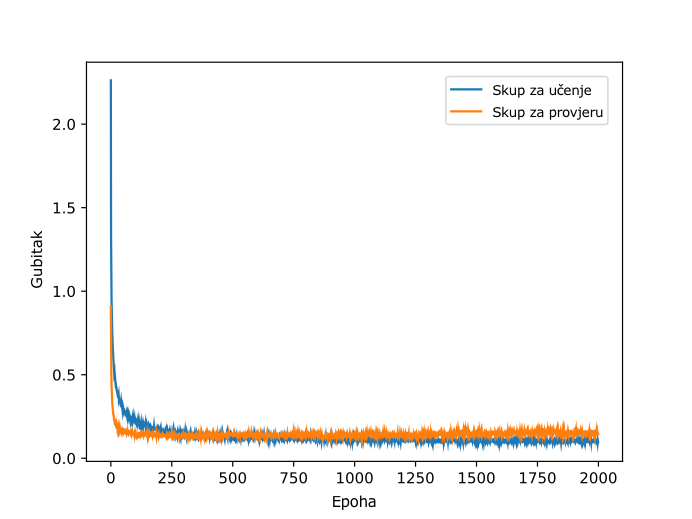
\includegraphics[width=10cm]{images/loss_prejoined.png}
    \caption{Gubitak modela}
    \label{fig:model_loss}
\end{figure}

\begin{figure}[!ht]
    \centering
    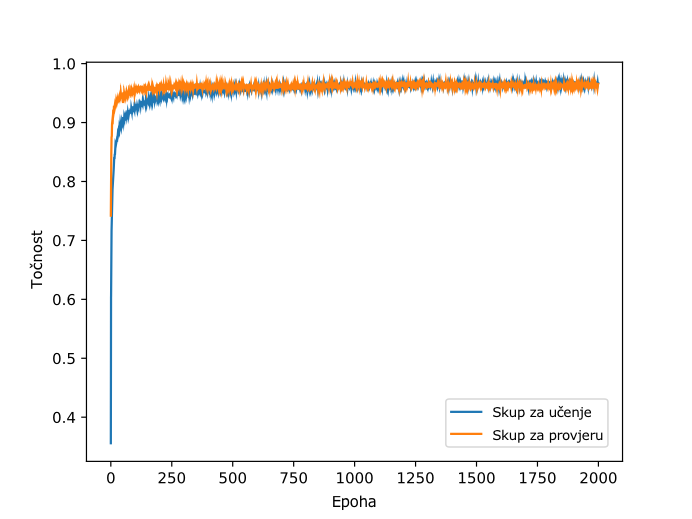
\includegraphics[width=10cm]{images/acc_prejoined.png}
    \caption{Točnost klasifikacije modela}
    \label{fig:model_acc}
\end{figure}

\section{Rezultati}

Najbolji rezultati su ostvareni na konvolucijskoj neuronskoj mreži opisanoj u prijašnjem poglavlju uz već navedene postupke učenja i tehnika regularizacije. Točnost klasifikacije modela na skupu za testiranje iznosila je $97.16 \%$ koja je postignuta nakon $1000$ epoha. Zatim se postupak učenja ponovio tako da se spoji skup za učenje te skup za provjeru na $1000$ epoha, te je postignuta konačna točnost modela na skupu za testiranje od $96.24 \%$. Prikaz vrijednosti funkcije gubitka takve mreže kroz epohe za pojedine skupove vidljiv je na slici \ref{fig:model_loss_joined}, dok se točnost klasifikacije kroz epohe može promatrati na slici \ref{fig:model_acc_joined}.

\begin{figure}[!ht]
    \centering
    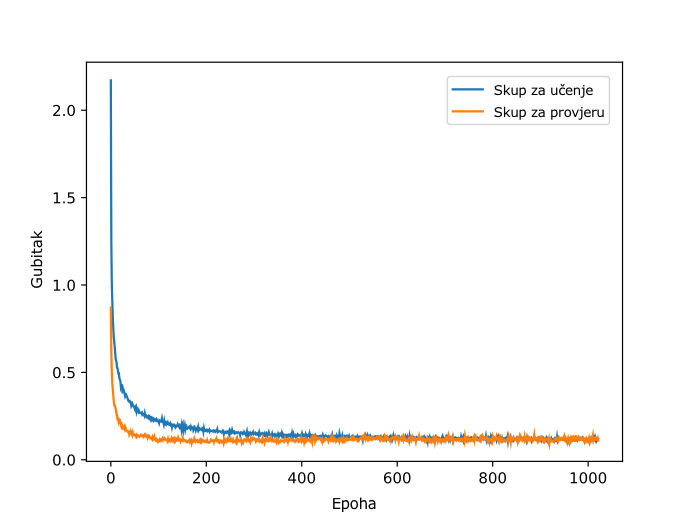
\includegraphics[width=9cm]{images/loss_joined.png}
    \caption{Gubitak modela}
    \label{fig:model_loss_joined}
\end{figure}

\begin{figure}[!ht]
    \centering
    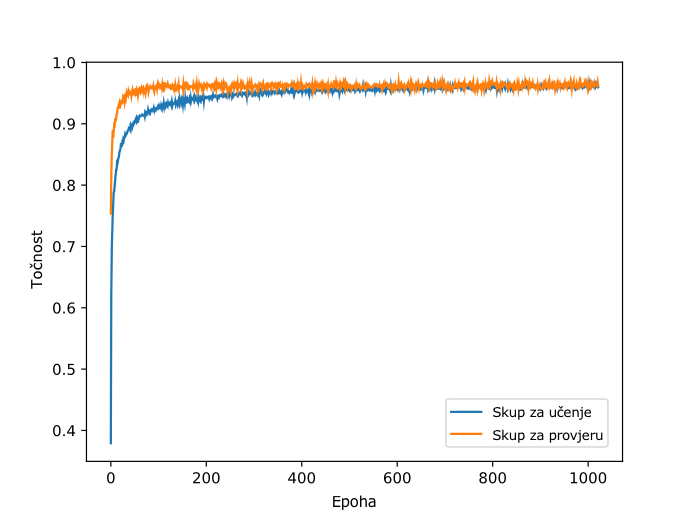
\includegraphics[width=9cm]{images/acc_joined.png}
    \caption{Točnost klasifikacije modela}
    \label{fig:model_acc_joined}
\end{figure}

Primjer krivo klasificiranih primjera iz skupa za ispitivanje vidljiv je na slici \ref{fig:wrong_class}. Može se uočiti kako najviše problema uzrokuju kombinacije malog slova l i velikog slova I, malog slova h i malog slova n te slova č i slova ć. No, među danim primjerima se mogu uočiti i krivo napisana slova, poput obrnutog slova N. Za velik broj slučajeva s navedene slike ni sam čovjek ne bi mogao točno razlučiti o kojem je slovu riječ bez poznavanja šireg konteksta u kojem se to slovo pojavilo.

\begin{figure}[htb]
    \centering
    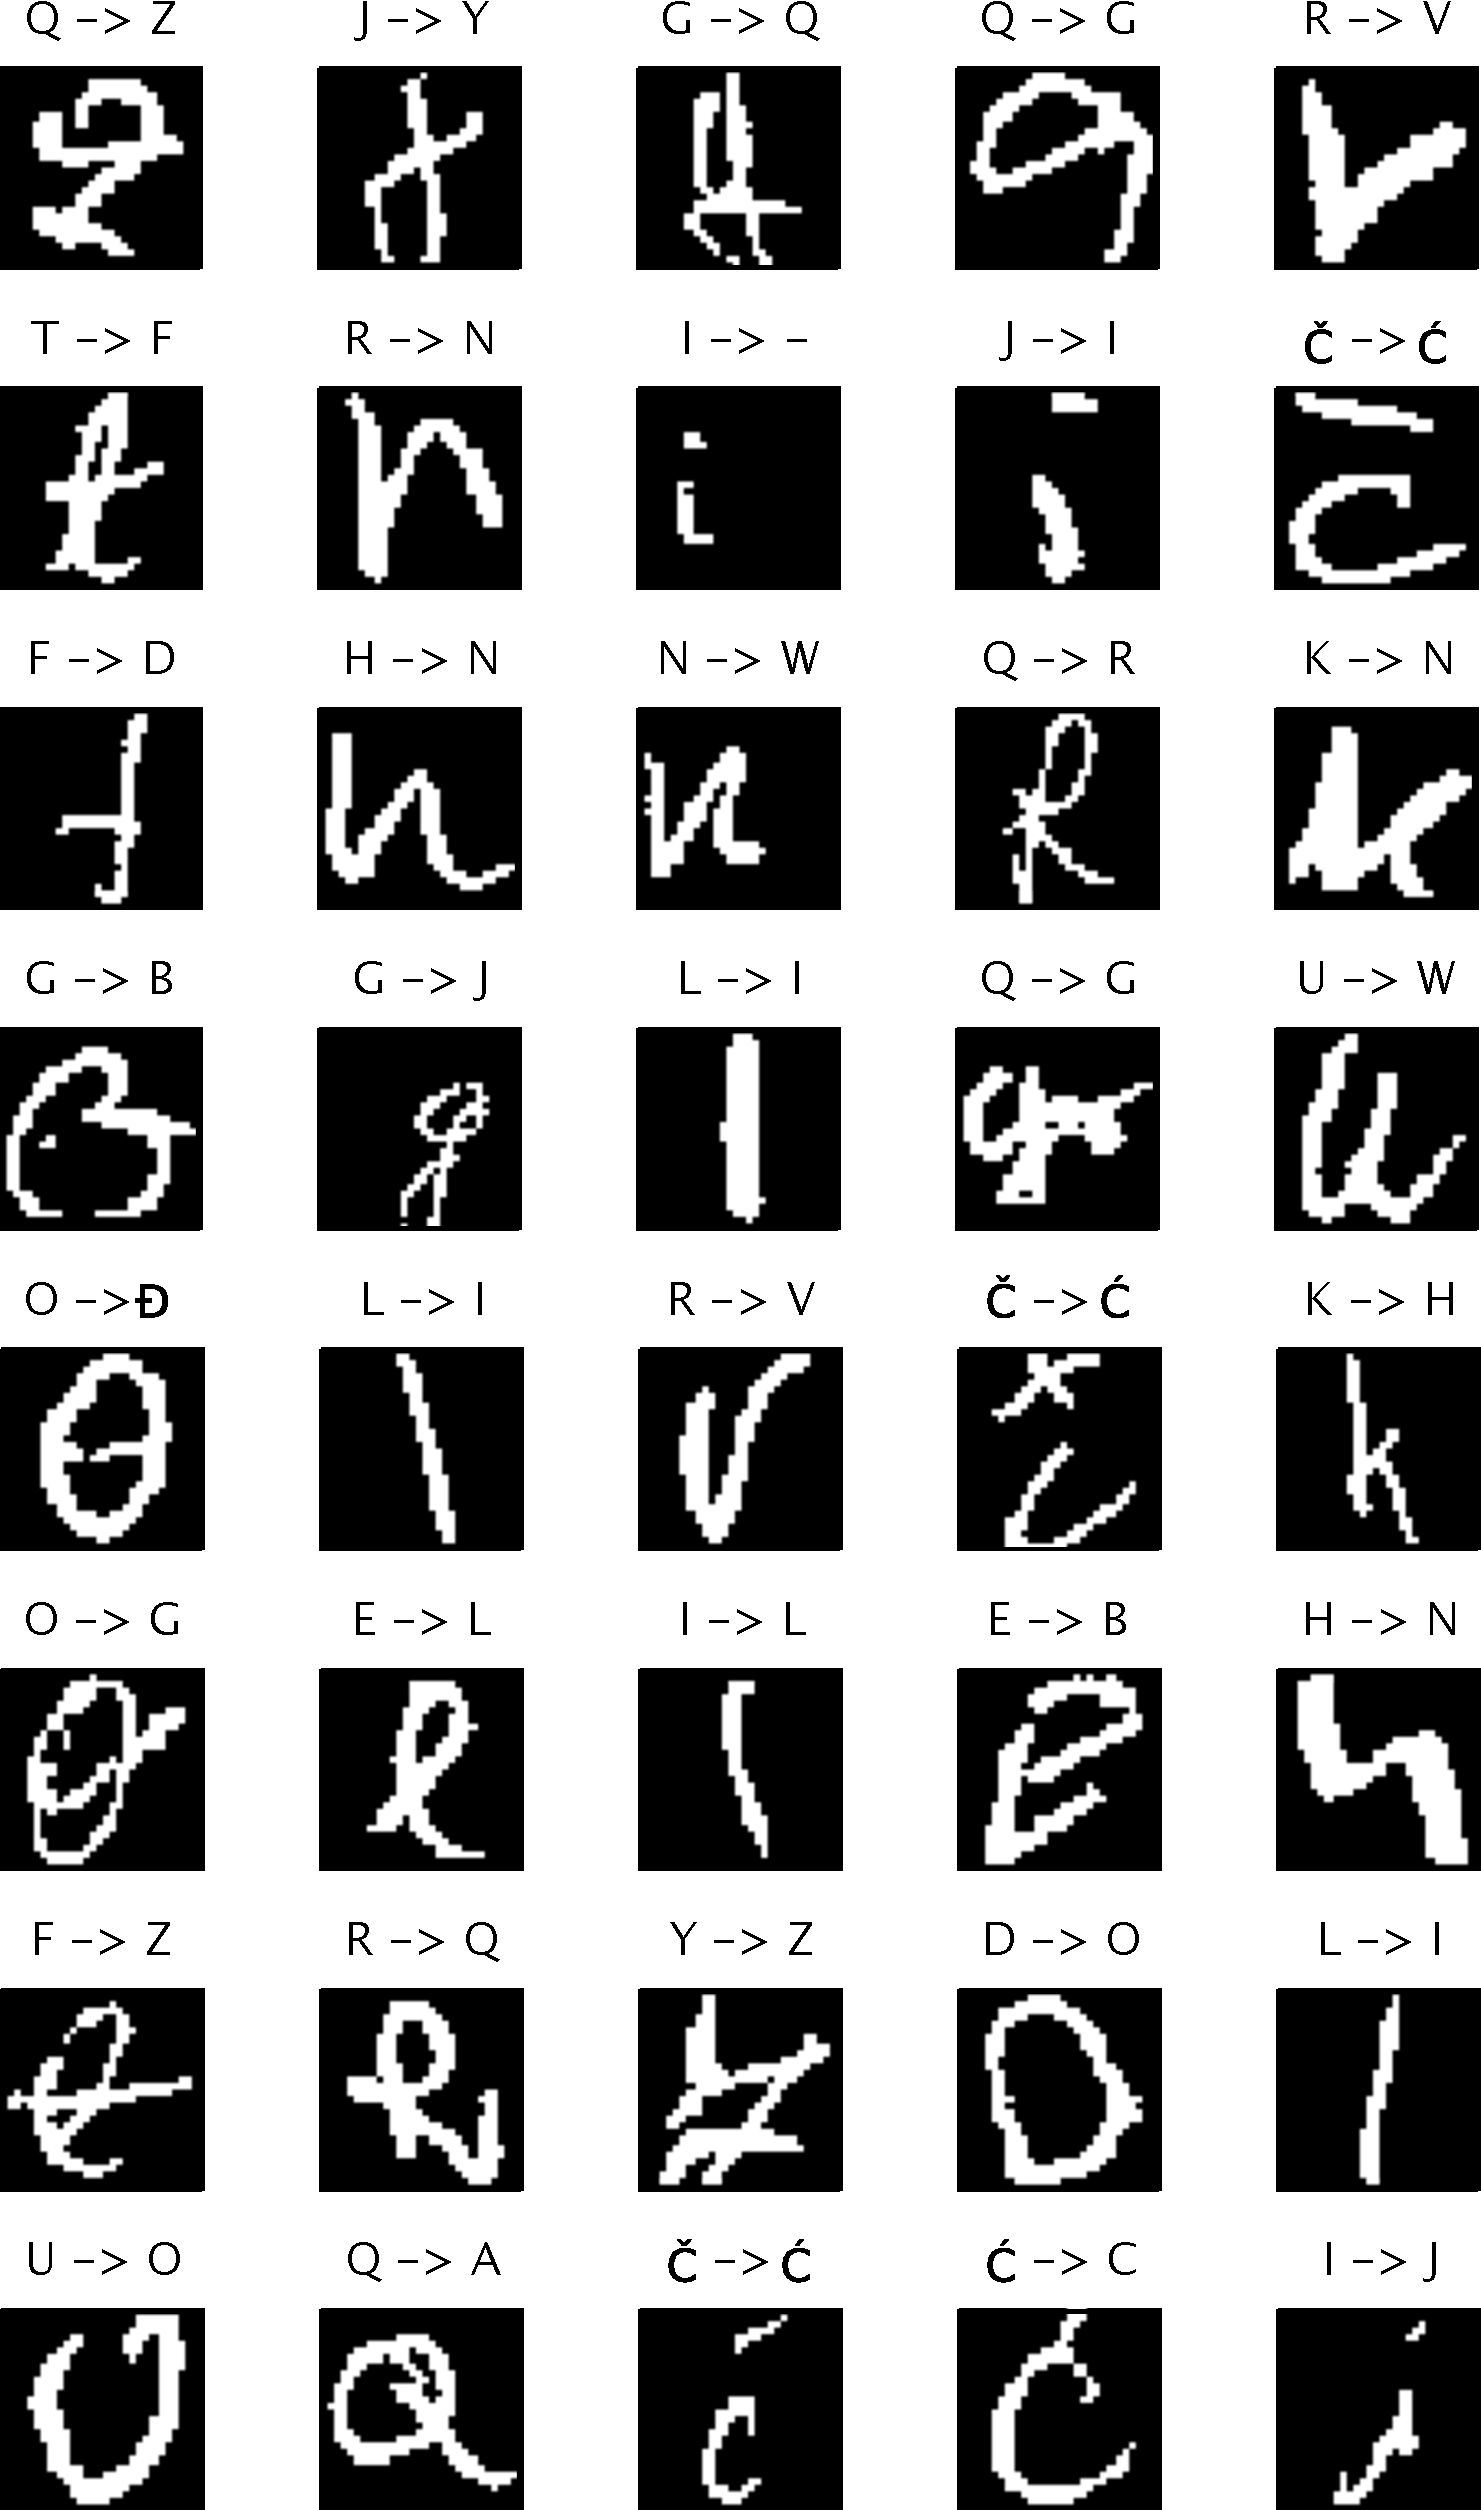
\includegraphics[width=9cm]{images/wrong_class.pdf}
    \caption{Krivo klasificirani primjeri iz skupa za ispitivanje. Lijeva strana izraza predstavlja stvarnu oznaku, a desna izlaz klasifikatora.}
    \label{fig:wrong_class}
\end{figure}

Tablicom \ref{confusion_matrix_cro} prikazana je matrica zabune na ispitnom skupu gdje pojedini element iz tablice predstavlja broj koliko je puta slovo iz retka prepoznato kao slovo iz stupca.
 
\begin{table}[]
\setlength{\tabcolsep}{2pt}
\centering
\caption{Matrica zabune za hrvatsku abecedu. Element tablice predstavlja broj koliko je puta slovo iz retka prepoznato kao slovo iz stupca.}
\label{confusion_matrix_cro}
\scalebox{0.8} {
\renewcommand{\arraystretch}{0.85}
\renewcommand{\tabcolsep}{0.5mm}
\begin{tabular}{|c|c|c|c|c|c|c|c|c|c|c|c|c|c|c|c|c|c|c|c|c|c|c|c|c|c|c|c|c|c|c|c|c|}
\hline  \rowcolor{gray1}
  & A & B & C & Č & Ć & D & Đ & E & F & G & H & I & J & K & L & M & N & O & P & R & S & Š & T & U & V & Z & Ž & X & Y & W & Q & -           \\ \hline 
A & \textbf{39} & 0 & 0 & 0 & 0 & 0 & 0 & 0 & 0 & 0 & 0 & 0 & 0 & 0 & 0 & 0 & 0 & 0 & 0 & 0 & 0 & 0 & 0 & 0 & 0 & 0 & 0 & 0 & 0 & 0 & 0 & 0           \\ \hline  \rowcolor{gray1}
B & 0 & \textbf{28} & 0 & 0 & 0 & 0 & 0 & 0 & 0 & 0 & 0 & 0 & 0 & 0 & 0 & 0 & 0 & 0 & 0 & 0 & 0 & 0 & 0 & 0 & 0 & 0 & 0 & 0 & 0 & 0 & 0 & 0           \\ \hline
C & 0 & 0 & \textbf{32} & 0 & 0 & 0 & 0 & 0 & 0 & 0 & 0 & 0 & 0 & 0 & 0 & 0 & 0 & 0 & 0 & 0 & 0 & 0 & 0 & 0 & 0 & 0 & 0 & 0 & 0 & 0 & 0 & 0           \\ \hline \rowcolor{gray1}
Č & 0 & 0 & 0 & \textbf{27} & 3 & 0 & 0 & 0 & 0 & 0 & 0 & 0 & 0 & 0 & 0 & 0 & 0 & 0 & 0 & 0 & 0 & 0 & 0 & 0 & 0 & 0 & 0 & 0 & 0 & 0 & 0 & 0           \\ \hline
Ć & 0 & 0 & 1 & 0 & \textbf{43} & 0 & 0 & 0 & 0 & 0 & 0 & 0 & 0 & 0 & 0 & 0 & 0 & 0 & 0 & 0 & 0 & 0 & 0 & 0 & 0 & 0 & 0 & 0 & 0 & 0 & 0 & 0           \\ \hline \rowcolor{gray1}
D & 0 & 0 & 0 & 0 & 0 & \textbf{31} & 0 & 0 & 0 & 0 & 0 & 0 & 0 & 0 & 0 & 0 & 0 & 1 & 0 & 0 & 0 & 0 & 0 & 0 & 0 & 0 & 0 & 0 & 0 & 0 & 0 & 0           \\ \hline
Đ & 0 & 0 & 0 & 0 & 0 & 0 & \textbf{33} & 0 & 0 & 0 & 0 & 0 & 0 & 0 & 0 & 0 & 0 & 0 & 0 & 0 & 0 & 0 & 0 & 0 & 0 & 0 & 0 & 0 & 0 & 0 & 0 & 0           \\ \hline \rowcolor{gray1}
E & 0 & 1 & 0 & 0 & 0 & 0 & 0 & \textbf{26} & 0 & 0 & 0 & 0 & 0 & 0 & 1 & 0 & 0 & 0 & 0 & 0 & 0 & 0 & 0 & 0 & 0 & 0 & 0 & 0 & 0 & 0 & 0 & 0           \\ \hline
F & 0 & 0 & 0 & 0 & 0 & 1 & 0 & 0 & \textbf{28} & 0 & 0 & 0 & 0 & 0 & 0 & 0 & 0 & 0 & 0 & 0 & 0 & 0 & 0 & 0 & 0 & 1 & 0 & 0 & 0 & 0 & 0 & 0           \\ \hline \rowcolor{gray1}
G & 0 & 1 & 0 & 0 & 0 & 0 & 0 & 0 & 0 & \textbf{29} & 0 & 0 & 1 & 0 & 0 & 0 & 0 & 0 & 0 & 0 & 0 & 0 & 0 & 0 & 0 & 0 & 0 & 0 & 0 & 0 & 1 & 0           \\ \hline
H & 0 & 0 & 0 & 0 & 0 & 0 & 0 & 0 & 0 & 0 & \textbf{32} & 0 & 0 & 0 & 0 & 0 & 2 & 0 & 0 & 0 & 0 & 0 & 0 & 0 & 0 & 0 & 0 & 0 & 0 & 0 & 0 & 0           \\ \hline \rowcolor{gray1}
I & 0 & 0 & 0 & 0 & 0 & 0 & 0 & 0 & 0 & 0 & 0 & \textbf{28} & 1 & 0 & 1 & 0 & 0 & 0 & 0 & 0 & 0 & 0 & 0 & 0 & 0 & 0 & 0 & 0 & 0 & 0 & 0 & 1           \\ \hline
J & 0 & 0 & 0 & 0 & 0 & 0 & 0 & 0 & 0 & 0 & 0 & 1 & \textbf{29} & 0 & 0 & 0 & 0 & 0 & 0 & 0 & 0 & 0 & 0 & 0 & 0 & 0 & 0 & 0 & 1 & 0 & 0 & 0           \\ \hline \rowcolor{gray1}
K & 0 & 0 & 0 & 0 & 0 & 0 & 0 & 0 & 0 & 0 & 1 & 0 & 0 & \textbf{28} & 0 & 0 & 1 & 0 & 0 & 0 & 0 & 0 & 0 & 0 & 0 & 0 & 0 & 0 & 0 & 0 & 0 & 0           \\ \hline
L & 0 & 0 & 0 & 0 & 0 & 0 & 0 & 0 & 0 & 0 & 0 & 3 & 0 & 0 & \textbf{40} & 0 & 0 & 0 & 0 & 0 & 0 & 0 & 0 & 0 & 0 & 0 & 0 & 0 & 0 & 0 & 0 & 0           \\ \hline \rowcolor{gray1}
M & 0 & 0 & 0 & 0 & 0 & 0 & 0 & 0 & 0 & 0 & 0 & 0 & 0 & 0 & 0 & \textbf{43} & 0 & 0 & 0 & 0 & 0 & 0 & 0 & 0 & 0 & 0 & 0 & 0 & 0 & 0 & 0 & 0           \\ \hline
N & 0 & 0 & 0 & 0 & 0 & 0 & 0 & 0 & 0 & 0 & 0 & 0 & 0 & 0 & 0 & 0 & \textbf{27} & 0 & 0 & 0 & 0 & 0 & 0 & 0 & 0 & 0 & 0 & 0 & 0 & 1 & 0 & 0           \\ \hline \rowcolor{gray1}
O & 0 & 0 & 0 & 0 & 0 & 0 & 1 & 0 & 0 & 1 & 0 & 0 & 0 & 0 & 0 & 0 & 0 & \textbf{33} & 0 & 0 & 0 & 0 & 0 & 0 & 0 & 0 & 0 & 0 & 0 & 0 & 0 & 0           \\ \hline
P & 0 & 0 & 0 & 0 & 0 & 0 & 0 & 0 & 0 & 0 & 0 & 0 & 0 & 0 & 0 & 0 & 0 & 0 & \textbf{33} & 0 & 0 & 0 & 0 & 0 & 0 & 0 & 0 & 0 & 0 & 0 & 0 & 0           \\ \hline \rowcolor{gray1}
R & 0 & 0 & 0 & 0 & 0 & 0 & 0 & 0 & 0 & 0 & 0 & 0 & 0 & 0 & 0 & 0 & 1 & 0 & 0 & \textbf{33} & 0 & 0 & 0 & 0 & 2 & 0 & 0 & 0 & 0 & 0 & 1 & 0           \\ \hline
S & 0 & 0 & 0 & 0 & 0 & 0 & 0 & 0 & 0 & 0 & 0 & 0 & 0 & 0 & 0 & 0 & 0 & 0 & 0 & 0 & \textbf{40} & 0 & 0 & 0 & 0 & 0 & 0 & 0 & 0 & 0 & 0 & 0           \\ \hline \rowcolor{gray1}
Š & 0 & 0 & 0 & 0 & 0 & 0 & 0 & 0 & 0 & 0 & 0 & 0 & 0 & 0 & 0 & 0 & 0 & 0 & 0 & 0 & 0 & \textbf{27} & 0 & 0 & 0 & 0 & 0 & 0 & 0 & 0 & 0 & 0           \\ \hline
T & 0 & 0 & 0 & 0 & 0 & 0 & 0 & 0 & 1 & 0 & 0 & 0 & 0 & 0 & 0 & 0 & 0 & 0 & 0 & 0 & 0 & 0 & \textbf{37} & 0 & 0 & 0 & 0 & 0 & 0 & 0 & 0 & 0           \\ \hline \rowcolor{gray1}
U & 0 & 0 & 0 & 0 & 0 & 0 & 0 & 0 & 0 & 0 & 0 & 0 & 0 & 0 & 0 & 0 & 0 & 1 & 0 & 0 & 0 & 0 & 0 & \textbf{33} & 0 & 0 & 0 & 0 & 0 & 1 & 0 & 0           \\ \hline
V & 0 & 0 & 0 & 0 & 0 & 0 & 0 & 0 & 0 & 0 & 0 & 0 & 0 & 0 & 0 & 0 & 0 & 0 & 0 & 0 & 0 & 0 & 0 & 0 & \textbf{35} & 0 & 0 & 0 & 0 & 0 & 0 & 0           \\ \hline \rowcolor{gray1}
Z & 0 & 0 & 0 & 0 & 0 & 0 & 0 & 0 & 0 & 0 & 0 & 0 & 0 & 0 & 0 & 0 & 0 & 0 & 0 & 0 & 0 & 0 & 0 & 0 & 0 & \textbf{40} & 0 & 0 & 0 & 0 & 0 & 0           \\ \hline
Ž & 0 & 0 & 0 & 0 & 0 & 0 & 0 & 0 & 0 & 0 & 0 & 0 & 0 & 0 & 0 & 0 & 0 & 0 & 0 & 0 & 0 & 0 & 0 & 0 & 0 & 0 & \textbf{32} & 0 & 0 & 0 & 0 & 0           \\ \hline \rowcolor{gray1}
X & 0 & 0 & 0 & 0 & 0 & 0 & 0 & 0 & 0 & 0 & 0 & 0 & 0 & 0 & 0 & 0 & 0 & 0 & 0 & 0 & 0 & 0 & 0 & 0 & 0 & 0 & 0 & \textbf{32} & 0 & 0 & 0 & 0           \\ \hline
Y & 0 & 0 & 0 & 0 & 0 & 0 & 0 & 0 & 0 & 0 & 0 & 0 & 0 & 0 & 0 & 0 & 0 & 0 & 0 & 0 & 0 & 0 & 0 & 0 & 0 & 1 & 0 & 0 & \textbf{26} & 0 & 0 & 0           \\ \hline \rowcolor{gray1}
W & 0 & 0 & 0 & 0 & 0 & 0 & 0 & 0 & 0 & 0 & 0 & 0 & 0 & 0 & 0 & 0 & 0 & 0 & 0 & 0 & 0 & 0 & 0 & 0 & 0 & 0 & 0 & 0 & 0 & \textbf{22} & 0 & 0           \\ \hline
Q & 1 & 0 & 0 & 0 & 0 & 0 & 0 & 0 & 0 & 2 & 0 & 0 & 0 & 0 & 0 & 0 & 0 & 0 & 0 & 1 & 0 & 0 & 0 & 0 & 0 & 1 & 0 & 0 & 0 & 0 & \textbf{24} & 0           \\ \hline \rowcolor{gray1}
- & 0 & 0 & 0 & 0 & 0 & 0 & 0 & 0 & 0 & 0 & 0 & 0 & 0 & 0 & 0 & 0 & 0 & 0 & 0 & 0 & 0 & 0 & 0 & 0 & 0 & 0 & 0 & 0 & 0 & 0 & 0 & \textbf{33} \\ \hline
\end{tabular}
}
\end{table}


\chapter{Primjena}
Opisani sustav svoju primjenu bi mogao naći u raznim situacijama: od ispravljanja ručno zapisanih odgovora na ispitu, do samog podsustava u sustavu za očitavanja rukom pisanoga teksta. U sklopu ovog projekta isprobana je integracija navedenoga sustava na mobilni uređaj \emph{Apple iPhone} sa zaslonom osjetljivim na dodir, gdje bi korisnik unosio tekst crtanjem slova na samom zaslonu.

\section{Pretvorba modela}

Kako je već spomenuto, za učenje klasifikatora konvolucijske neuronske mreže korišten je radni okvir \emph{Keras}. Navedeni okvir omogućava izlučivanje naučenoga modela i njegovih težina koji se kasnije mogu upotrebljavati u drugim radnim okvirima i programskim jezicima.

Jedan takav okvir je i \emph{Apple-ov} \emph{Core ML} \cite{coreml}. Navedeni okvir omogućava uključivanje i uporabu naučenih modela iz raznih okvira, poput \emph{Keras}, \emph{Xgboost}, \emph{scikit-learn} i drugih, na \emph{Apple-ovim} uređajima, što uključuje širok spektar: od pametnih satova, preko mobilnih uređaja do osobnih računala.

Posebnost navedenoga okvira je što se naučeni modeli nalaze na uređaju te su optimirani za izvođenje na prijenosnim uređajima gdje potrošnja energije i resursa mora biti što manja.

Radni okvir \emph{Core ML} je pisan u programskom jeziku \emph{Swift} te u pozadini koristi sljdeće radne okvire:
\begin{itemize}
  \item \emph{Accelerate} - optimirane matrične i vektorske operacije
  \item \emph{BNNS} - skup funkcija za lakše implementiranje neuronskih mreža
  \item \emph{Metal Performance Shaders} - izvođenje računskih operacija na \emph{GPU-u}
\end{itemize}

Postupak pretvorbe \emph{Keras} modela se obavljao koristeći službeni \emph{Appleov} alat \emph{coremltools} pisan u programskom jeziku \emph{Python}. Program kao parametar prima opis modela u definiranom \emph{JSON} formatu i njegove težine, te na izlazu vraća \emph{ML model} koji se zatim može koristiti na \emph{Appleovim} \emph{iOS} i \emph{macOS} sustavima.

\section{Aplikacija}

Za potrebe ovog rada napisana je aplikacija imena \emph{SmartLetter} u programskom jeziku \emph{Swift}. Grafičko sučelje navedene aplikacije prikazano je na slici \ref{fig:app}. Korisnik dodirom i potezima crta slovo na platnu te aplikacija ispisuje prepoznato slovo. Samo prepoznavanje znaka traje ispod jedne milisekunde, a to obuhvaća: pretprocesiranje ulaznog znaka (izvlačenje okvira, centriranje i skaliranje), pretvorba u crno-bijelu sliku, propuštanje kroz konvolucijsku neuronsku mrežu te na kraju obradu izlaza mreže, to jest ispis prepoznatog znaka.

\begin{figure}[htb]
    \centering
    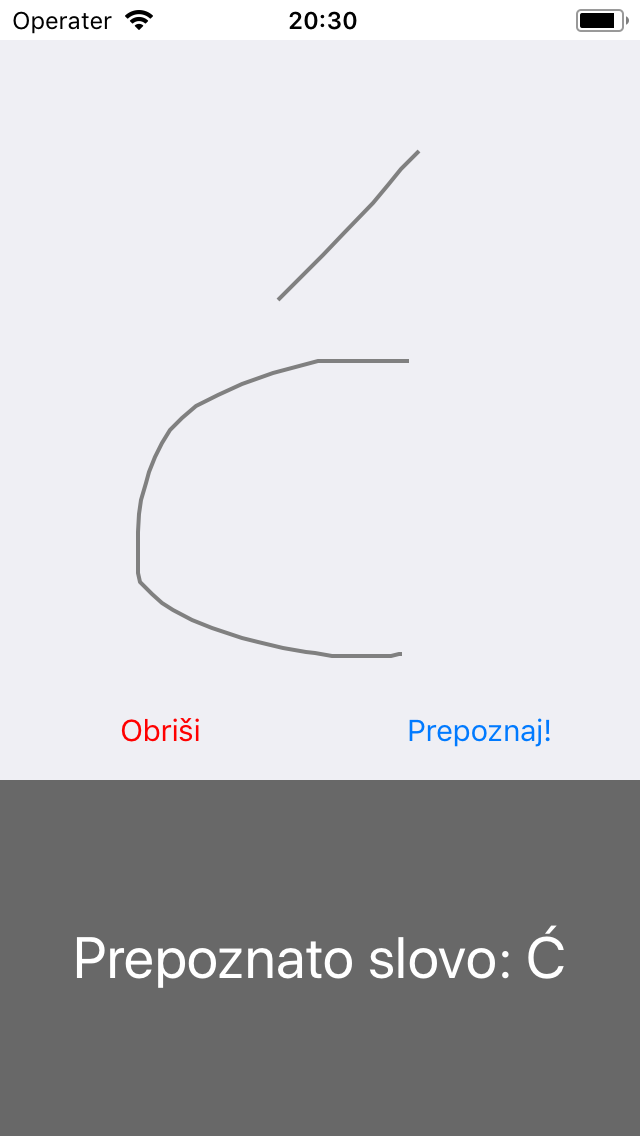
\includegraphics[width=6cm]{images/app2.png}
    \caption{\emph{SmartLetter} aplikacija.}
    \label{fig:app}
\end{figure}

Kako sama aplikacija i nema neku svrhu osim isprobavanja sustava za prepoznavanje znakova, implementirana je dodatna komponenta aplikacije, to jest tipkovnica koja se može koristiti kroz cijeli \emph{iOS} sustav. Tipkovnica i primjer korištenja je prikazan na slici \ref{fig:keyboard}. Korisnik unosi tekst crtanjem na platnu. S lijeve strane je dugme za izmjenu velikih i malih slova, jer kako je već napomenuto, sustav na izlazu ima $32$ razreda, to jest združena pojedina velika i mala slova proširene hrvatske abecede. Na desnoj strani je dugme za brisanje prethodno napisanoga slova te prelazak u novi red. Za sam razmak se koristi posebni znak crtice "-".

Kako bi unos teksta bio što brži, ne koristi se posebno dugme za prepoznavanje već se prati kad je korisnik završio s crtanjem, to jest podignuo prst sa zaslona te se zatim vrši prepoznavanje. Navedeni pristup ima problem kod znakova koji su sastavljeni od više odvojenih dijelova, poput znakova č, ć, ž i sličnih jer korisnik mora podići prst kako bi nacrtao drugi dio znaka. Kao riješenje implementirana je odgoda prepoznavanja gdje sama aplikacija čeka određeno vrijeme idući unos, te ukoliko se ne dogodi tek onda vrši prepoznavanje znaka, a ako se dogodi onda samo nastavi iscrtavanje na već prije iscrtani znak. Isprobano je više intervala čekanja, no to uvelike ovisi o samo korisniku i njegovoj spretnosti prilikom pisanja. Najbolje vrijeme čekanja isprobanih na nekolicini korisnika je ispalo između $300$ i $600$ milisekundi.

\begin{figure}[htb]
    \centering
    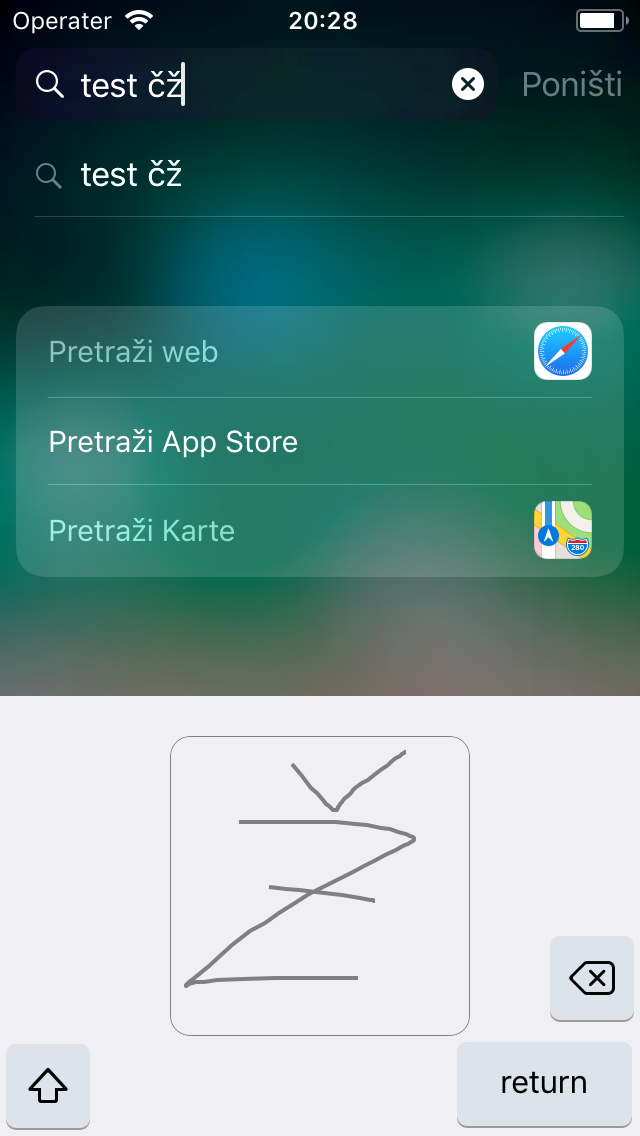
\includegraphics[width=6cm]{images/app1.png}
    \caption{\emph{SmartLetter} tipkovnica u sustavu \emph{iOS}.}
    \label{fig:keyboard}
\end{figure}



\chapter{Zaključak}
Tehnika očitavanja rukom pisanih slova se razvija još od polovice prošlog stoljeća i od tada je u mnogočemu evoluirala. U ovom radu, kao klasifikator pojedinog slova, korištena je konvolucijska neuronska mreža.

U radu je predstavljen cjeloviti postupak prikupljanja skupa podataka i obrade slike kako bi se ulazna slika pripremila za svrhu učenja konvolucijske neuronske mreže. Također, opisana je arhitektura korištene neuronske mreže i postupak učenja iste.

Dobivena je točnost od $96.24 \%$ na skupu za ispitivanje, što je poboljšanje preko $2 \%$ u odnosu na točnost dobivenu u radu \cite{seminar} koja je iznosila $94 \%$. U navedenom radu je korištena nešto složenija arhitektura konvolucijske neuronske mreže te sličan skup podataka za učenje koji nije bio pročišćen.

Također, u radu je prikazana i primjena navedenoga modela u vidu aplikacije, odnosno tipkovnice za \emph{Appleov iOS} sustav koja se kod niza korisnika pokazala iznimnom dobrom, intuitivnom i jednostavnom za korištenje. Osobni dojam korisnika je bila i iznimna preciznost samog sustava prepoznavanja, što je vrlo dobro uzevši u obzir da je model učen na znakovima pisanim rukom na papiru gdje je dolazilo do gubitaka informacije u samom pretprocesiranju slike.

Za budući rad bi se isti taj sustav mogao isprobati i na manjim uređajima poput pametnih satova gdje fizički nije moguće smjestiti običnu tipkovnicu na zaslonu.

\bibliography{literatura}
\bibliographystyle{fer}

% \chapter{Sažetak}
% U ovom radu opisana je implementacija i način rada sustav za očitavanje rukom pisanih slova koji je projektiran tako da na svoj ulaz primi sliku slova dimenzija $30 \times 30$, a na svom izlazu vrati prepoznato slovo. Sam sustav je zasnovan na konvolucijskoj neuronskoj mreži učenu metodom \emph{Adam}. Skup za učenje konvolucijske neuronske mreže se sastojao od \num{12,141} velikih i malih tiskanih slova hrvatske i engleske abecede te znaka ''-''. Točnost klasifikatora provjerena je na skupu za ispitivanje koji se sastojao od \num{1063} znaka te je iznosila $96,24 \%$.

\end{document}
